\chapter{Learning Vector Quantization}
\label{chapter:intro}
\section{簡介}

	%%圖\ref{fig:lvq_network}爲LVQ的網路架構圖。SOM是一個分群的演算法,如果將它的概念轉成監督式學習,就是LVQ演算法的由來。這個演算法可用於分類的應用,且具有簡單的架構。

	學習向量量化(Learning Vector Quantization,簡稱爲LVQ),可以將其視爲是一種人工神經網路的特例。
	圖\ref{fig:lvq_network}爲LVQ的網路架構圖。
	從圖中可以發現這個網路僅具有輸入與輸出兩層,所以是一個結構相當簡單的神經網路,並且是一個具有監督式學習的分類演算法。
	此外,在這個演算法中,採取了非監督式學習的機制,應用於監督式學習的問題上。

	\begin{figure}[h]
			\centering
			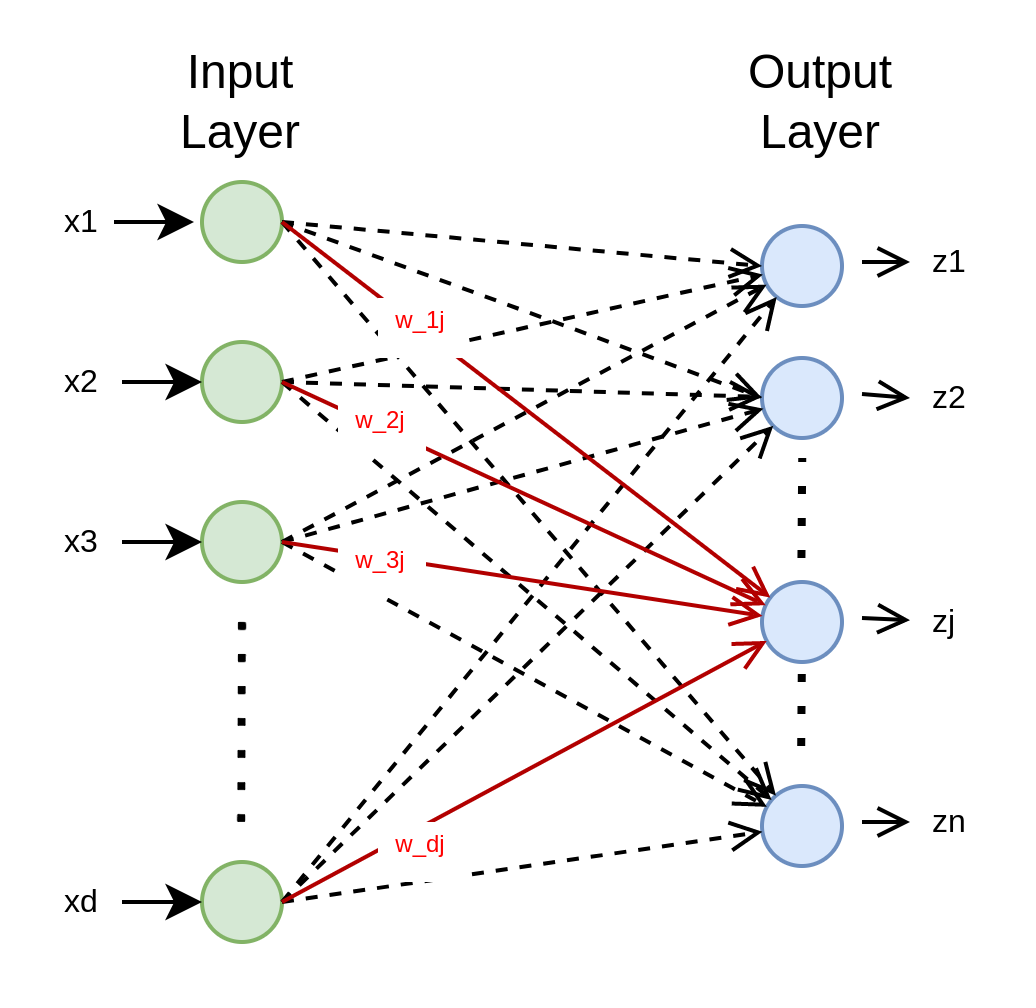
\includegraphics[height=10cm]{./pic/zMBsAkkS.png}
			\caption{LVQ網路架構圖}
			\label{fig:lvq_network}
	\end{figure}

\label{sec:background}


    \section{Vector Quantization}
		在理解LVQ演算法前,我們先來看看Vector Quatization。這個算法的目的主要是將原資料分割k個域區,並在這些分割的區域中,找出一個最能代表整個群組的向量,作為這個區域中的代表點。
		這些代表點的集合我們稱爲codebook。
		此外這個算法所做的事情有點類似將資料進行分群。


		從圖\ref{fig:data_after_vq},可以看到原資料被分割成3個區域,以及3個紅色方點,而紅色方點就是整個分割區域中的代表點,也是LVQ中的weight vetcor。


        \begin{figure}[h]
            \begin{center}
                \begin{tabular}{ccccccccccccc}
                    \subfigure[原資料集分佈]{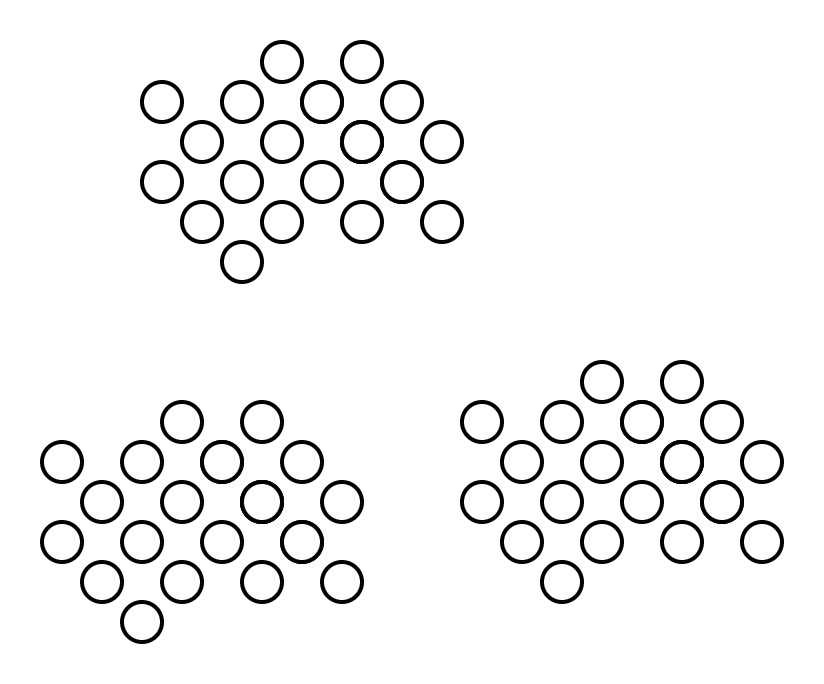
\includegraphics[height=4cm]{./pic/oA5nFv7C.png}\label{fig:ori_data} } \par &
                    \subfigure[經過向量量化的原資料]{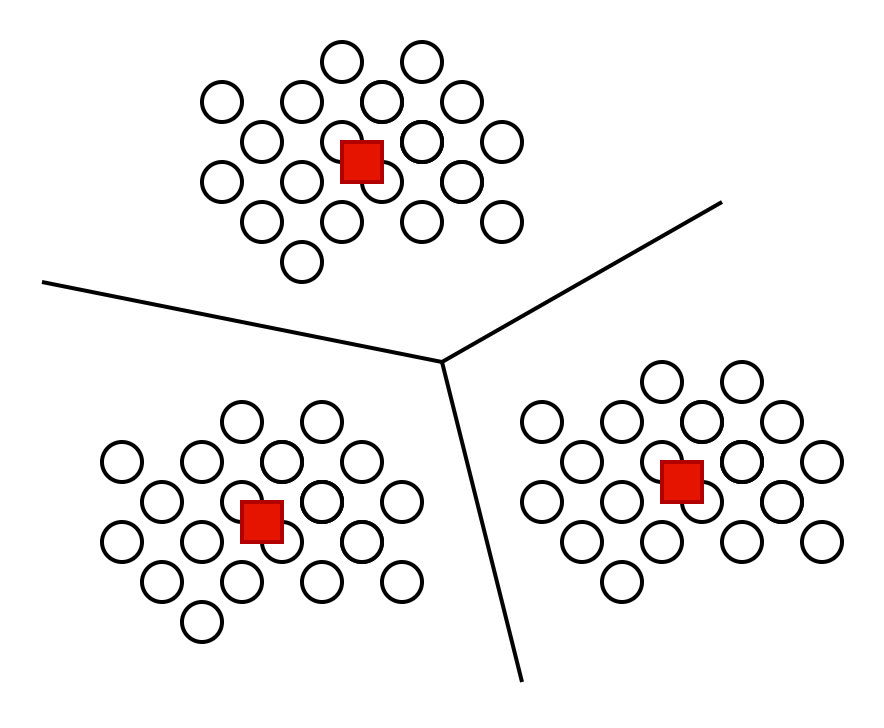
\includegraphics[height=4cm]{./pic/aLVdIIWU.png}\label{fig:data_after_vq} } \par \\
                \end{tabular}
                \caption{向量量化的示意圖}
                \label{fig:vector_quantization}
            \end{center}
        \end{figure}


%%- 權重向量爲,$$\mathbf{w_{j}} = (w_{1j},w_{2j},w_{3j},....,w_{nj})$$
%%- 距離的計算採用,尤拉距離公式 $$D(j)=||\mathbf{x}-\mathbf{w_j}||_2 = \sqrt{(x_1-w_{1j})^2+(x_2-w_{2j})^2+...+(x_n-w_{nj})^2} $$
%%- $$C_j$$ 為網路層的輸出類別。
%%- $$T$$ 為每筆資料所對應的實際類別。
%%- $$\alpha$$爲學習率


\section{演算法參數定義與流程}

	%%在這個演算法中只有Input Layer與Output Layer

	\subsection{參數定義}

    \begin{itemize}
        \item
			輸入向量,\(\mathbf{x} = (x_1,x_2,x_3,....,x_d)\),爲資料集中的其中一筆資料。

        
        %
        \item
			權重,\(\mathbf{W} = (\mathbf{w_1,w_2,...,w_j,...w_d})\),爲一個 \(d \times n \)的矩陣,也就是剛剛介紹Vector Quantization所提到的codebook。 
        %
        \item
			權重向量,\(\mathbf{w_{j}} = (w_{1j},w_{2j},w_{3j},....,w_{dj})\),代表每個區域的代表點。
        
        %
        \item
			\(D(j)\)爲每筆資料與代表點的距離。
			$$D(j)=||\mathbf{x}-\mathbf{w_j}||_2 = \sqrt{(x_1-w_{1j})^2+(x_2-w_{2j})^2+...+(x_n-w_{nj})^2} $$


        \item
		\(C_j\) 為網路層的輸出類別。

		\item
		\(\alpha\) 爲學習率
		 
    \end{itemize}


\subsection{流程}

首先會先初始化 \(\mathbf{W},\alpha\),接著將所有的訓練資料集中的每一筆資料,找出與每筆資料最近權重向量,並接著判斷 \(C_j\) 的結果是否符合這筆資料的類別,如果相同就使得這個權重向量靠近這筆資料點且更新學習率,反之,如果不同則遠離。接著不斷重複以上步驟,直到訓練次數或是學習率達到設定的標準,則停止模型訓練。下圖爲演算法的流程圖\ref{fig:alogrithm_workflow}。

\newpage

\usetikzlibrary{positioning, shapes.geometric}

\tikzset{every picture/.style={line width=1.75pt}}


	\begin{figure}
	\resizebox{300pt}{400pt}{
		\begin{tikzpicture}[scale=1]
			\node[draw, rounded corners,align=center ]                        (start)   {初始化參數 \(\mathbf{W},\alpha\) };
		  \node[draw,diamond, below=20pt of start,align = center]                        (step 2)  {訓練 \(\mathbf{x}\) 中的\\每一筆資料};
		  \node[draw,  aspect=2, below=20pt of step 2]     (step 3)  {找出 \(min\{D(1),D(2),...,D(j),..D(d)\}\) };
		  \node[draw, diamond,below=20pt of step 3]                   (compare)  {比對 \(C_j\)與 \(T\)  };
		  \node[draw, below =30pt of compare,align = center]                         (same)  {\(\mathbf{w_j(new)} = \mathbf{w_j(old)} + \alpha(\mathbf{x} - \mathbf{w_j(old)})\)  };
		  \node[draw, below right=55pt and 80pt of compare]                         (different)  {\(\mathbf{w_j(new)} = \mathbf{w_j(old)} - \alpha(\mathbf{x} - \mathbf{w_j(old)})\)};
		  \node[draw, rounded corners, below=20pt of same]  (learning_rate)     {更新學習率 \(\alpha\) };
		  \node[draw,diamond, below=20pt of learning_rate,align = center]                         (end_detect)  {判斷是否\\達到結束條件};
		  \node[draw, rounded corners, below=20pt of end_detect]  (end)     {End};
		  
		  \draw[->] (start)  --coordinate(le) (step 2);
		  \draw[->] (step 2) --node[left]{Yes} (step 3);
		  \draw[->] (step 2.west) --node[above]{Yes}++(-50pt,0)|-(end_detect.west);
		  \draw[->] (step 3) -- (compare);
		  \draw[->] (compare) -> node[left]{Yes}(same.north);
		  \draw[->] (compare.east) --node[above]{No}(compare.east-|different.north) -> (different.north);
		  \draw[->] (same) -- (learning_rate);
		  \draw[->] (learning_rate) -> (end_detect);
		  \draw[->] (end_detect) -- node[left]{Yes}(end);
		  \draw[->] (end_detect.east) --node[above]{No}++(250pt,0pt)|-(le) ;
		
		\end{tikzpicture}
		}
		\caption{演算法流程圖}
		\label{fig:alogrithm_workflow}
	\end{figure}







    %要被單行註解的文字。

\begin{comment}
    要被區塊註解的文字,要被區塊註解的文字,要被區塊註解的文字,
    要被區塊註解的文字,要被區塊註解的文字,要被區塊註解的文字,
    要被區塊註解的文字,要被區塊註解的文字,要被區塊註解的文字,
    要被區塊註解的文字,要被區塊註解的文字,要被區塊註解的文字,
    要被區塊註解的文字,要被區塊註解的文字,要被區塊註解的文字,
    要被區塊註解的文字,要被區塊註解的文字。
\end{comment}

\section{研究動機與目的}
    動機與目的,動機與目的,動機與目的,動機與目的,
    動機與目的,動機與目的,動機與目的,動機與目的,
    動機與目的,動機與目的,動機與目的,動機與目的,
    動機與目的,動機與目的,動機與目的,動機與目的,
    動機與目的,動機與目的,動機與目的,
    細節如表\ref{tab:mytitle1}。

    \begin{enumerate}
        \item
        列舉一。
        %
        \item
        列舉二。
        %
        \item
        列舉三。
        %
    \end{enumerate}

\section {研究方法與論文架構}
    研究方法與論文架構,研究方法與論文架構,研究方法與論文架構,
    研究方法與論文架構,研究方法與論文架構,研究方法與論文架構,
    研究方法與論文架構,研究方法與論文架構,研究方法與論文架構,
    研究方法與論文架構。

    \begin{itemize}
        \item
        項目一。
        %
        \item
        項目二。
        %
        \item
        項目三。
        %
        \item
        項目四。
    \end{itemize}

    流程圖如\ref{fig:ResearchFlowChart}。
    \begin{figure}[htbp]
        \centering
        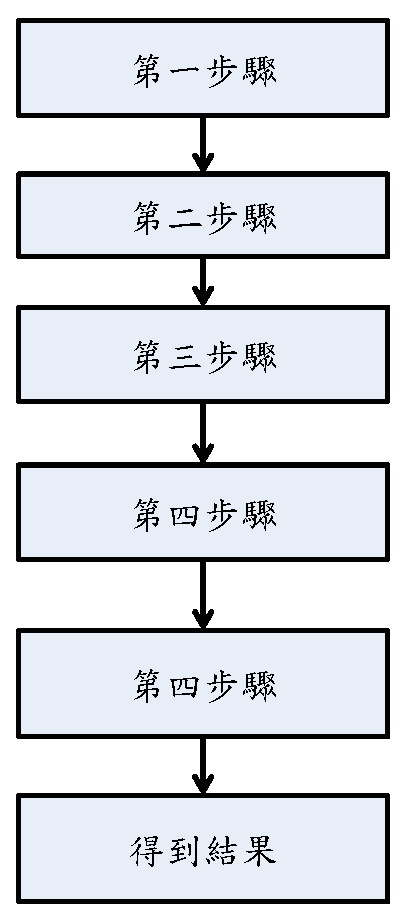
\includegraphics[height=8cm]{graphs/introduction/ResearchFlowChart.eps}
        \caption{研究進行流程圖}
        \label{fig:ResearchFlowChart}
    \end{figure}

